\section{Methodology}
\label{sec_methodology}

%To evaluate the contribution of thermal and high energy neutrons to the error rate of devices it is necessary to: (1) measure the probability that a neutron will generate a fault, and (2) estimate the flux of high energy and thermal neutrons where the device will operate. 
%We measure (1) through accelerated neutron beams experiments and estimate (2) using existing data as well as initial measurements of actual thermal neutron rates in an approximate setting.

In this section, we describe the devices and applications chosen to test the impact of high energy and thermal neutrons in modern computing devices reliability. We also detail the radiation experiments setup used for this work and describe the detector we used to measure the impact of materials in the thermal neutron flux.

\subsection{Devices}
\label{subsec_devices}

We selected six devices for this study using different technologies and vendors to have an in-depth insight of thermal neutrons sensitivity on a breadth of modern devices. It is worth noting that both the fabrication process and the foundry can significantly impact the amount of $^{10}B$ in the device.

\textbf{Intel Xeon Phi} is designed for HPC systems, built using a \textbf{$22nm$ Intel's 3-D Tri-gate technology}.

\textbf{NVIDIA K20} is a GPU built with the $Kepler$ architecture and fabricated in a \textbf{$28nm$ TSMC CMOS technology}.

\textbf{NVIDIA TitanX} is a GPU built with the $Pascal$ architecture and fabricated in a \textbf{$16nm$ TSMC FinFET technology}.

\textbf{NVIDIA TitanV} is built with the $Volta$ architecture and fabricated in a \textbf{$12nm$ TSMC FinFET technology}.

\textbf{AMD Accelerated Processing Unit (APU)} integrates CPU and GPU in the same chip fabricated in a \textbf{$28nm$ SHP Bulk Process at Global Foundries}.

\textbf{FPGA} is the Zynq-7000 designed by Xilinx using a \textbf{$28nm$ TSMC technology}.

%\textbf{Intel Xeon Phi} is an HPC accelerator that, even if recently announced as dismissed, powers some of the fastest supercomputers from the Top500 list~\cite{Dongarra2013}. The Xeon Phi tested is the coprocessor 3120A, which implements the $Knights\:Corner$ architecture, and it is built using a \textbf{$22nm$ Intel's 3-D Tri-gate technology}.  
%
%\textbf{NVIDIA K20} is a GPU built with the $Kepler$ architecture and is fabricated in a \textbf{$28nm$ TSMC standard CMOS technology}. This model is specially built for HPC systems and has 2496 CUDA cores divided across 15 Streaming Multiprocessors (SMs). 
%
%\textbf{NVIDIA TitanX} is a GPU built with the $Pascal$ architecture and fabricated in a \textbf{$16nm$ TSMC FinFET}, it has 3584 CUDA cores split across 28 SMs. 
%
%\textbf{NVIDIA TitanV} is built with the $Volta$ architecture and fabricated in a \textbf{$12nm$ TSMC FinFET}, it features 5120 CUDA cores divided into 80 SMs. 
%
%\textbf{AMD Accelerated Processing Unit (APU)} is a heterogeneous device that integrates CPU and GPU in the same chip sharing the same memory. The APU considered is the AMD A10 7890K Kaveri fabricated in a \textbf{$28nm$ SHP Bulk Process at Global Foundries}. This device includes 4 Steamroller CPU cores and a GCN architecture AMD Radeon R7 Series GPU containing 512 cores with 866MHZ each. 
%We consider three APU configurations: CPU, GPU, and CPU+GPU. 
%
%\textbf{FPGA} is the Zynq-7000 designed by Xilinx using a \textbf{$28nm$ TSMC technology}. The FPGA is composed mainly of Configurable Logic Blocks (CLBs), Digital Signal Processor (DSP) blocks, and embedded memory blocks (BRAM). 


\subsection{Codes}
\label{subsec_codes}

The set of devices we consider covers a wide range of architectural and computational characteristics. Using the same code for each device would bias the reliability evaluation, in favor of the devices that are more efficient in executing the chosen code. 
To have a fair evaluation, then, we choose for each class of devices the codes that better fit with its computational characteristics. For Xeon Phi and GPUs we chose four codes representative of \textbf{HPC}: MxM, LUD, LavaMD, and HotSpot. We selected three \textbf{heterogeneous} codes specially made to fully utilize the APU architecture: SC, CED, and BFS. Finally, on GPUs and FPGA we tested two \textbf{neural networks} to represent codes that  have a significant impact on self-driven vehicles: YOLO and MNIST. 

\textbf{Matrix Multiplication (MxM)} is representative of highly arithmetic compute-bound codes used in HPC and for features extraction in CNNs~\cite{Dongarra2013}. 

\textbf{LUD} is a linear algebra method that calculates solutions for a square system of linear equations.%, representative of highly compute-bound codes~\cite{lava2009}. 

\textbf{LavaMD} simulates particle interactions using Finite Difference Methods~\cite{lava2009}. %LavaMD is compute bound, being mostly composed of dot-products. 

\textbf{Hotspot} is representative of stencil solvers~\cite{lava2009}, it estimates the processor temperature using an architectural
floor plan and simulated power measurements. 

\textbf{Stream Compaction (SC)} is a memory-bound code used in databases and image processing applications. SC is composed of a data manipulation primitive that removes elements from an array.

\textbf{Canny Edge Detection (CED)} extracts information from images and reduce the amount of data to be processed. CPU and GPU concurrently work on different frames. %The input frames are a subset of the Urban Dataset used for neural networks training \cite{fragkiadaki2012two}. 

\textbf{Breadth First Search (BFS)} is a search in graphs algorithms that performs non-uniform memory access widely used in GPS Navigation Systems. 
%The input graph we select for our evaluation represents the highways of the Great Lakes area in the US \cite{DIMACS} 

\textbf{YOLO} is a Convolution Neural Network (CNN) used for object classification and detection~\cite{yolo2015}. 

\textbf{MNIST} is a CNN used for classifying handwritten digits~\cite{deng2012}. We have tested MNIST only on FPGAs as it is a minimal network that would not exercise sufficient resources on GPUs or Xeon Phis.


\subsection{Radiation Experiments Setup}
\label{sub_beam_setup}

\begin{figure}[tb]
\centering
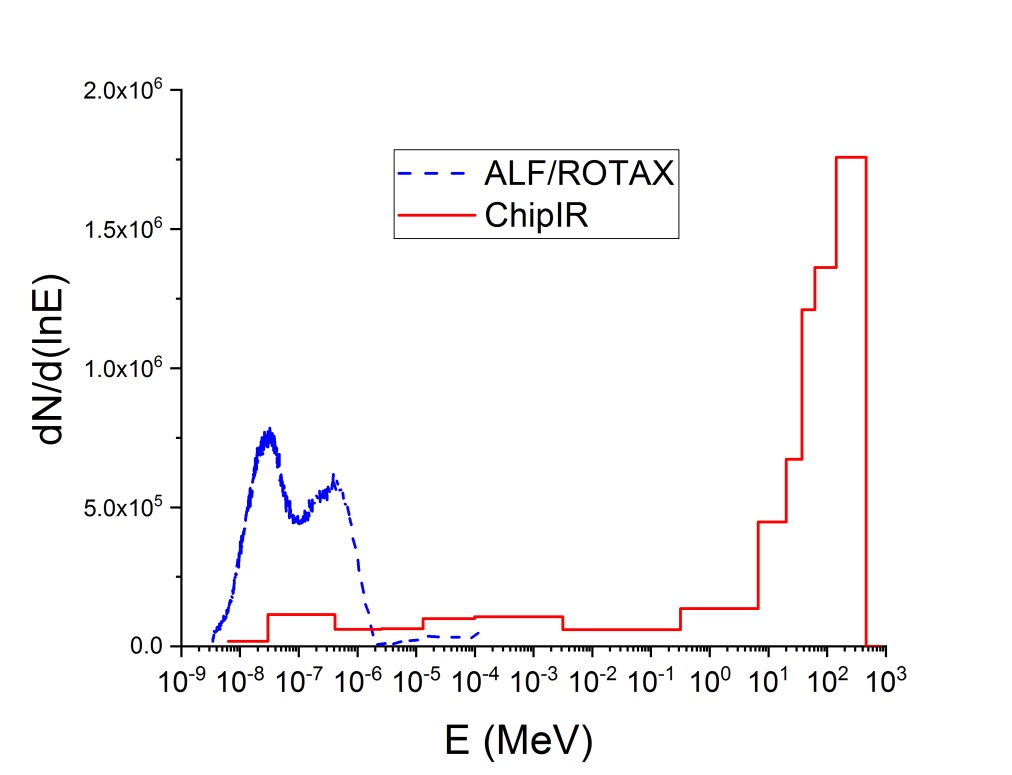
\includegraphics[width=0.35\textwidth]{./figs/rotax-chipir}
\caption{The neutron spectra of the beamlines used for irradiation in lethargy scale.}
\label{rotax_chipir}
\end{figure}

To evaluate the sensitivity of our devices to high energy and thermal neutrons we exposed the devices on two different beamlines at the ISIS spallation neutron source in the UK: ChipIR for high energy neutrons and ROTAX for thermal neutrons.
ChipIR~\cite{cazzaniga2018progress} is the reference beamline dedicated to the irradiation of microelectronics and it features a high energy neutron spectrum, as similar as possible to the atmospheric one. The flux with neutron energy above 10 MeV is $5.4 \times {10}^6 n/{cm}^2/s$, while the thermal component ($E < 0.5 eV$) is $4 \times {10}^5 n/{cm}^2/s$~\cite{chiesa2018measurement}.
ROTAX~\cite{tietze1989rotax} is a general purpose beamline with a thermal neutron spectrum generating a flux of $2.72\times{10}^6 n/{cm}^2/s$. Here the thermalization is achieved by moderation of the neutrons using liquid methane. 

The spectra of the two beamlines are compared in Figure~\ref{rotax_chipir} on a log-log scale where the fluxes are proportional to the areas under the curves. As Figure~\ref{rotax_chipir} suggests, most neutrons in ROTAX are thermals and most neutron in ChipIR are high energy one.

%To evaluate the sensitivity to thermal and high energy neutrons we align the devices described in Section~\ref{subsec_devices} with the beam, while executing the codes listed in Section~\ref{subsec_codes}. The device output is compared with a pre-computed fault-free copy and any mismatch is marked as an SDC. If the application dies, gets stuck, or the device stops responding we count this as a DUE. Dividing the number of observed errors with the fluence the device has received we can calculate the device sensitivity, expressed as \textbf{cross section} [$cm^2$]. 
%The higher the cross section, the higher the probability for one neutron (either thermal or high energy) to generate an observable error (either SDC or DUE). 
%
%To eliminate any setup-dependent differences between thermal and high energy neutrons, we irradiate the 
%same physical devices executing the codes with the same input vector both in ROTAX and in ChipIR. It is worth noting that, apart from DDR that experienced permanent faults, testing the same device at ROTAX and then at ChipIR (or the other way around) does not influence the measured error rates.
%The only difference between the two experiments is that, thanks to the higher neutron energies, at ChipIR we can align various boards with the beam, as shown in Figure~\ref{rad_setup}. Using a derating factor that takes distance into account we can measure the sensitivity of multiple devices in parallel. In ROTAX, as the irradiate devices stop most of the incoming thermal neutrons, we must test one device at a time. In Figure~\ref{rad_setup} we show the setup for the Titan V evaluation. 

To evaluate the sensitivity to thermal and high energy neutrons we align the devices with the beam, while executing the codes. The device output is compared with a pre-computed fault-free copy and any mismatch is marked as an SDC. If the device stops responding we count a DUE.  To eliminate any setup-dependent differences between thermal and high energy neutrons, we irradiate the same physical devices executing the codes with the same input both in ROTAX and in ChipIR. The only difference between the two experiments is that at ChipIR we can align various boards with the beam, as shown in Figure~\ref{rad_setup}. Using a derating factor that takes distance into account we can measure the sensitivity of multiple devices in parallel. In ROTAX, as the irradiate device block most of the incoming neutrons, we must test one device at a time.
%Due to limitations in the thermal neutrons experiment, we could only test one sample of each device. The high energy neutrons error rate variation among different samples of the same device has already been shown to be low, recent works indicate a variation of about 10\%~\cite{sc2017,Oliveira2017}. 


%\begin{figure}[tb]
%\centering
%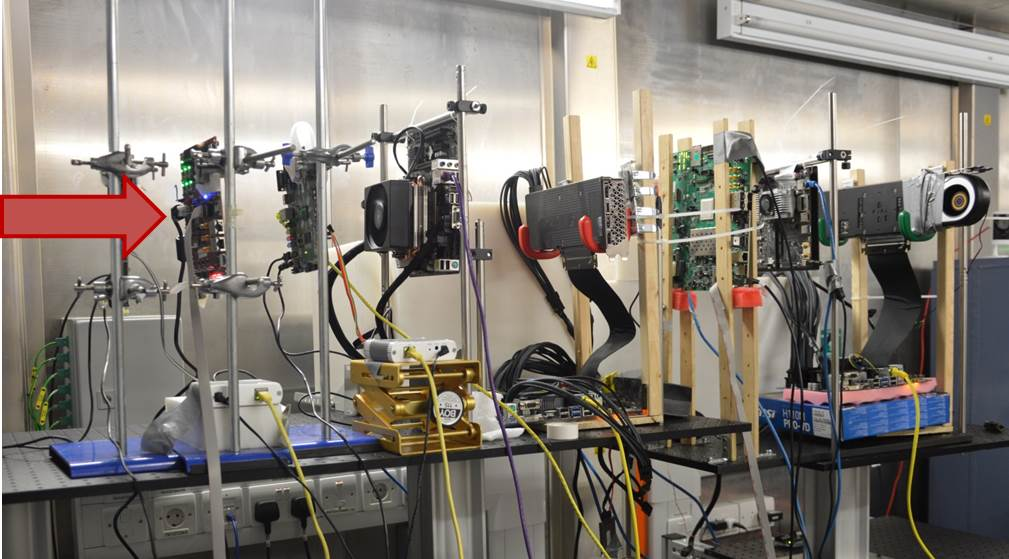
\includegraphics[width=0.90\columnwidth]{./figs/ChipIR_setup}
%\caption{Experimental setup in ChipIR. The arrow indicates the direction of the neutron beam.}
%\label{ChipIR_setup}
%\end{figure}
%
%
%\begin{figure}[tb]
%\centering
%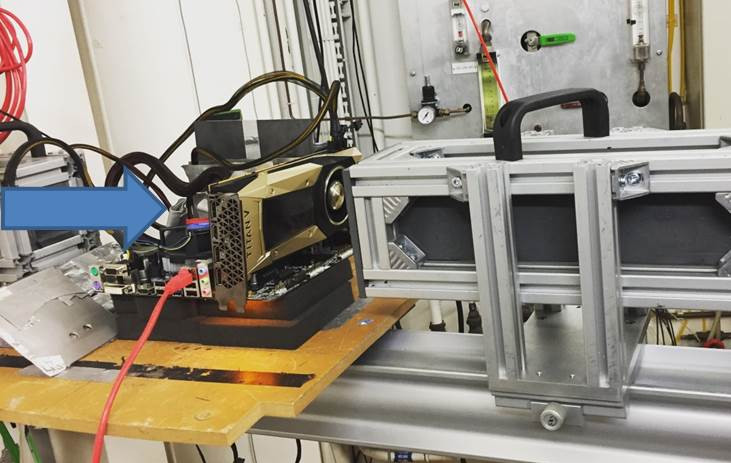
\includegraphics[width=0.9\columnwidth]{./figs/Rotax_setup}
%\caption{Titan X experimental setup in ROTAX. The arrow indicates the direction of the thermal neutron beam.}
%\label{rotax_setup}
%\end{figure}
\begin{figure}[tb]
\centering
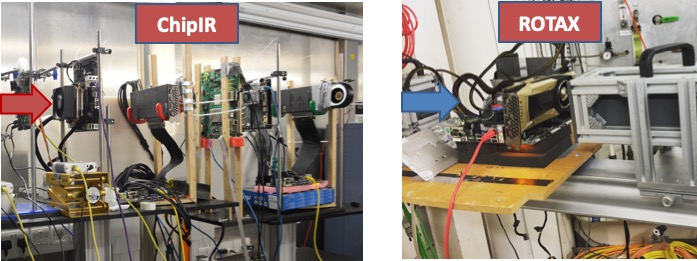
\includegraphics[width=0.80\columnwidth]{./figs/setup}
\caption{Experimental setup in ChipIR and ROTAX. The arrow indicates the direction of the neutron beam.}
\label{rad_setup}
\end{figure}


\subsection{Thermal Neutrons Detector}
\label{sub_detector}


We have designed and deployed a thermal neutron detector, called Tin-II, to measure the flux of thermal neutrons in different conditions. Ultimately, Tin-II will be used to measure the flux of thermal neutrons inside the data center housing the Trinity supercomputer at LANL. %Tin-II consists of two identical $^{3}He$ cylindrical detectors. The interaction of radiation (neutrons, gammas, betas, etc.) with the detectors triggers a reaction that is amplified, filtered, and counted as an event.

%We calibrated the two detectors for a period of 18 hours to ensure that they have the same detection efficiency. Then, we shielded one of the two cylinders with cadmium. Cadmium effectively blocks thermal neutrons, while being  transparent to  other types of radiation such as high energy neutrons, gammas, betas, etc. As a result, one of the two cylinder (bare detector) detects all radiation reactions, while the other (shielded detector) counts only radiation reactions that are not thermal neutrons. The difference in count rates between these two detectors, multiplied by an efficiency value, reflects the average thermal neutron flux.

Tin-II counted thermal neutron events over the course of several days. To estimate the effect of some of the characteristic materials in modern data centers on the thermal neutron flux, we placed a box containing 2 inches of water close to the detector. The count difference with and without the water, shown in details in Section~\ref{sub_flux}, indicates its influence in the thermal neutrons flux.


